% This is the Oregon State University LaTeX template. To the best of my
% knowledge, most of the work was done by those acknowledged in beavtex.cls.

%%
%% Preamble
%%
% \documentclass{<something>} must begin each LaTeX document
\documentclass[double,12pt]{beavtex}
% Added by CII
\usepackage{graphicx,latexsym, array, wrapfig}
\usepackage{amsmath}
\usepackage{amssymb,amsthm}
\usepackage{longtable,booktabs,setspace}
\usepackage[hyphens]{url}
\usepackage[colorlinks = true, 
			urlcolor = blue,
			linkcolor = black,
			citecolor = black,
			anchorcolor = black]{hyperref}
\usepackage{lmodern}
\usepackage{float}
\floatplacement{figure}{H}
% End of CII addition
\usepackage{rotating} % Package added to allow the rotation of figures and chart
                      % on a page, {sidewaysfigure} command
\usepackage{tablefootnote} % Packaged added to allow footnotes in the tabular
                           % environment, use \tablefootnote command

% This has to do with a default pandoc thing
% http://tex.stackexchange.com/a/258486/77699
\providecommand{\tightlist}{%
  \setlength{\itemsep}{0pt}\setlength{\parskip}{0pt}}

% Added by CII (Thanks, Hadley!)
% Use ref for internal links
\renewcommand{\hyperref}[2][???]{\autoref{#1}}

\def\sectionautorefname{Section}
\def\subsectionautorefname{Subsection}
% End of CII addition

% Added by CII
\usepackage{caption}
\captionsetup{width=5in}
% End of CII addition

\title{Response of Stream Macroinvertebrate Community to Canopy-opening
Manipulations} % {An Analysis of Something}
\author{Cedar Mackaness} % {Joseph A. Student}
\degree{Honors Baccalaureate of Science} % {Master of Science}
\doctype{Thesis}
\submitdate{November 15, 2019} % {January 1, 2013}
\commencementyear{2020} % {2013}

\department{Environmental Science} % {Nuclear Engineering and Radiation Health Physics}

\depttype{College of Earth, Ocean and Atmospheric Sciences} % {School}

\depthead{Dave Lytle} % {Director}

\major{Environmental Science} % {Radiation Health Physics}

\advisor{Dana Warren} % {Jane R. Professor}

\abstract{Stream light availability is an important factor influencing aquatic
food webs. In forested headwaters, stream algal production is often
highly light-limited, so an increase in light enhances benthic algal
growth, which in turn increases food availability for primary consumers
in the stream. In forested headwater streams, light availability is
almost entirely mediated by the canopy structure of stream-side
vegetation. Over the last century, many streamside forests in the
Pacific Northwest were heavily harvested, leading to dense regenerating
stands along streams today. Under current conditions, the dense closed
canopies, allow for limited primary production, and we hypothesize that
low standing stocks of benthic primary producers under these closed
canopy forests lead to a low abundance of invertebrates that feed on
stream algae. We investigated the reach-scale responses of benthic
periphyton, stream macroinvertebrates, and prey consumption by trout to
a localized release from light limitation in a paired-reach study
design. We expected that increases in light availability would promote
elevated algal production causing the invertebrate community to shift
toward scraper dominance, and predicted that this change in community
structure is detectable in the diets of trout. In contrast to our
expectations, we found that the presence of a canopy gap had little
influence on the invertebrate community, and this lack of change was not
being masked by increased consumption of grazing invertebrates in summer
trout diets.}
\acknowledgements{I would like to thank Allison Swartz, Dana Warren and the whole Warren
lab for several years of sometimes-grueling-always-fun work, and the
opportunity and support to work on this thesis project. Additionally, I
would like to acknowledge both Dave Roon and Dave Lytle, my thesis
committee members, for their novel insights and unique perspective. The
parts of this thesis that I am most proud of came about through
collaboration with all of the people mentioned above, and of course it
was all made possible through the love and encouragement of my family.}




	\dedication{For Kate and Matt, they got me this far\ldots{}}




\begin{document}

\maketitle
\mainmatter


  \chapter*{Introduction}\label{introduction}
  \addcontentsline{toc}{chapter}{Introduction}
  
  In forested systems, streams and their biota are intrinsically linked to
  riparian vegetation (Vannote, Minshall, Cummins, Sedell, \& Cushing,
  \protect\hyperlink{ref-Vannote1980}{1980}). Stream food webs depend on
  direct carbon subsidies from the terrestrial environment in the form of
  both leaf litter and terrestrial invertebrates (Wipfli,
  \protect\hyperlink{ref-Wipfli1997}{1997}), but riparian controls on
  stream systems aren't limited to organic inputs. Riparian canopy cover
  also has an indirect effect on stream food webs by limiting light
  available for benthic primary production. In the Pacific Northwest (PNW)
  region of North America, riparian forests have changed substantially in
  the past half century. In response to a legacy of heavy harvesting (Pan
  et al., \protect\hyperlink{ref-Pan2011}{2011}), riparian forest
  protections have created dense regenerating vegetation along streams in
  contrast with structurally complex old-growth forests containing
  multiple canopy gaps that historically dominated the PNW landscape (D.
  R. Warren et al., \protect\hyperlink{ref-Warren2016Eco}{2016}). The
  dense vegetation in these regenerating forests decreases light
  availability and limits benthic primary production {[}M. J. Kaylor,
  Warren, \& Kiffney (\protect\hyperlink{ref-Kaylor2017FS}{2017})). As
  forest stand development continues natural disturbances and individual
  tree mortalities will increase canopy heterogeneity through the
  introduction of gaps. To understand how aquatic food webs respond to an
  increase in light associated with canopy gaps, we investigate the
  response of macroinvertebrates and fish feeding to canopy-opening
  manipulations.
  
  Light, and its impact on primary productivity in streams is of
  particular interest because autochthonous carbon can be
  disproportionately represented in consumer biomass relative to its
  availability in aquatic systems (Lau, Leung, \& Dudgeon,
  \protect\hyperlink{ref-Lau2009}{2009}; McCutchan \& Lewis,
  \protect\hyperlink{ref-McCutchan2002}{2002}). In forested headwaters
  specifically, basal carbon availability is dominated by leaf litter
  (McCutchan \& Lewis, \protect\hyperlink{ref-McCutchan2002}{2002});
  however, energetically, algae is a higher quality food source and is
  preferentially assimilated into higher trophic levels (Macarelli,
  Baxter, Mineau, \& Hall Jr,
  \protect\hyperlink{ref-Macarelli2011}{2011}). Primary consumers mediate
  basal carbon availability for higher trophic levels and, in temperate
  streams, primary consumers are dominated by macroinvertebrates, a major
  food resource for insectivorous fish. Because macroinvertebrates play a
  crucial role in mediating food web interactions, understanding their
  community dynamics and functional diveristy can provide key insights
  into broader ecosystem and food web functioning. Invertebrates in the
  scraper functional feeding group in particular have evolved specialized
  mouthparts for consuming benthic algal biofilms (periphyton), and
  increases in algal production in high light areas are expected to elicit
  a positive response among these scraping taxa (Liess, Le Gros,
  Wagenhoff, Townsend, \& Matthaei,
  \protect\hyperlink{ref-liess2012}{2012}).
  
  Macroinvertebrate community data have traditionally been used to
  evaluate stream health. Indicies such as the B-IBI (benthic index of
  biological integrity) rely on total taxa richness and taxa richness of
  key families, such as Ephemeroptera, Plecoptera and Trichoptera (EPT
  taxa) to evaluate the biological condition of streams. Other indicies
  such as the EPT index focus on proportional abundance of taxa known to
  be sensitive to environmental disturbances. More broadly, an assessement
  of the whole community can be used to evaluate overall food web and
  ecosystem responses to a multitude of variables. For example, studies
  using nonmetric multidimensional scaling (NMS) have assessed community
  responses along a variety of environmental gradients (M. B. Cole,
  Russell, \& Mabee, \protect\hyperlink{ref-Cole2003}{2003}; Purcell et
  al., \protect\hyperlink{ref-Purcell2009}{2009}). The relationship
  between the synthetic community variables represented by the ordination
  axes and environmental variables provide a valuable tool for assessing
  overall community response to environmental factors.
  
  In headwater streams, the benthic invertebrate community represents the
  primary food source for trout. Interspecific interactions between trout
  and invertebrates can alter the benthic community as trout foraging
  (Dahl, \protect\hyperlink{ref-Dahl1998}{1998}), or fish presence alters
  the behavior of, or actively selects against, invertebrates vulnerable
  to trout predation (Peckarsky \& McIntosh,
  \protect\hyperlink{ref-Peckarsky1998}{1998}). Depending on the taxa
  present, top-down pressures on the invertebrate community may relieve
  algae from invertebrate grazing and ultimately increase benthic biofilm
  standing stock. In headwater streams trout are oportunistic foragers,
  and consumption tends to be biased toward large invertebrates.
  Additionally, cutthroat trout, the dominant fish species in Cascade
  headwaters, are visual predators typically feeding from the water
  column. Because salmonids are visual predators, their feeding efficiency
  can be influenced by visibility (Wilzbach, Cummins, \& Hall,
  \protect\hyperlink{ref-Wilzbach1986}{1986}), which is dependent on light
  conditions. Therefore, gaps have the potential to affect fish feeding
  not only through potential increases in scraper invertebrate food
  resources, but also by increasing foraging capture rates of all taxa and
  functional feeding groups. We expect the oportunistic nature of trout
  diets to reflect changes in the benthic community due to increases in
  primary production.
  
  While some studies on forest clearing have demonstrated that there can
  be reach-scale increase in benthic primary producers, invertebrates, and
  even trout when the system is released from light limitation (Murphy \&
  Hall, \protect\hyperlink{ref-Murphy1981}{1981}; Wootton,
  \protect\hyperlink{ref-Wootton2012}{2012}), harvesting without
  streamside buffers consistently leads to increases in temperature,
  losses of large wood habitat, and increases in stream sediment loads.
  Increased temperatures, increased sediment loading, and reduced habitat
  complexity can be detrimental to many headwater species. Given these
  negative impacts, clear-cutting adjacent to streams is no longer a
  common practice in the PNW and many streams have riparian buffers that
  maintain some stream shading. The streamside forests that are recovering
  from stand replacing clearing or from natural stand-replacing events
  over the past century are currently in the early-to-middle stages of
  development with dense homogenous canopy cover and low stream light
  (Kaylor et al. 2017). Canopy gaps will begin developing naturally along
  streams as stands mature, and restoration efforts focused on emulating
  natural disturbance may expedite forest shifts toward late-succession
  and old-growth structural conditions (Kreutzweiser, Sibley, Richardson,
  \& Gordon, \protect\hyperlink{ref-Kreutzweiser2012}{2012}). With
  riparian forest protections, we expect regenerating streamside stands to
  continue to develop more complex structure and eventually progress
  toward late successional forest structure with localized light patches
  of light associated with canopy gaps becoming increasingly prevalent.
  Similarly, in management areas with narrow buffers we still expect a
  dynamic light environment associated with upland cutting as an open
  understory lets in low-angle light. Whether due to natural stand
  development, efforts to increase forest structural complexity, or
  patches of shade along a stream created by thinner buffers, we expect
  the light environment of forested streams to become patchier in the
  coming years. While effects of large changes in canopy cover
  (i.e.~cutting all or nearly all of the riparian forest) have been
  studied in a number of cases, the more moderate influence of small
  canopy gaps and light patches on stream ecosystems has not been widely
  investigated, especially in an experimental context.
  
  We implemented a two-year before-after, control-impact study designed to
  detect and capture the effect of canopy gaps on aquatic
  macroinvertebrate communities. In this work, we expected that primary
  production would increase when canopy gaps were created, and this would
  cause the invertebrate community to shift toward more taxa in the
  scraper feeding group. However, we expected the reach-scale responses to
  a localized increase in light to be dampened in comparison to observed
  responses in large scale riparian clearing studies. In addition to
  evaluating benthic macroinvertebrate community, we also assessed trout
  diets to determine whether shifts in the invertebrate community would be
  reflected proportionally in the diet of opportunistic foraging of trout.
  The diet data were also used to evaluate whether a potential benthic
  invertebrate community response may be masked by increased selective
  foraging of particular taxa by these apex consumers.
  
  \chapter*{Methods}\label{methods}
  \addcontentsline{toc}{chapter}{Methods}
  
  \section*{Study location}\label{study-location}
  \addcontentsline{toc}{section}{Study location}
  
  The study consisted of five reach pairs on five replicate streams in the
  western Cascade Mountains of Oregon. Each reach pair consisted of one
  treatment reach and one reference reach. Two of the reach pairs (W-100,
  W-113) were located on private Weyerhaeuser Co. land, and three (LOON,
  CHUCK, MCTE) are located on U.S. Forest Service land, one of which
  (MCTE) was situated in the H.J. Andrews Experimental Forest. Stream
  reaches were 90 meters in length and treatment gaps were 20 to 40 meters
  in diameter and situated approximately around meter thirty of treatment
  reaches. Sites had a buffer between stream reach pairs to limit any
  effects of the upstream reach on downstream conditions.
  
  All of the streams are wadeable, fish-bearing streams with bankfull
  widths of 1-6 meters. Fish-bearing streams were purposefully selected to
  provide management-relevant results for key species such as salmonids.
  Additionally, low-order streams of this size range comprise up to 70\%
  of total stream length in forested catchments. The streams run through
  40 to 60-year-old riparian forests regenerating from previous harvest.
  These early-to-mid-seral stage forests have a homogenous canopy
  structure with heavy understory shading. Small streams also provide ease
  of sampling and maximize the effect of a canopy opening manipulation
  since small streams may be completely shaded by overhead vegetation.
  
  \begin{table}[t]
  
  \caption{\label{tab:table1}Study site attributes}
  \centering
  \resizebox{\linewidth}{!}{
  \begin{tabular}{lrrrrr}
  \toprule
  Stream & Elevation (m) & Bankful Width (m) & Base flow (L s-1) & Latitude & Longitude\\
  \midrule
  CHUCK & 833 & 5.20 & 21.0 & 43.95362 & -122.1136\\
  LOON & 721 & 4.13 & 12.5 & 43.95362 & -122.1833\\
  MCTE & 867 & 2.20 & 5.0 & 44.25454 & -122.1667\\
  W-100 & 441 & 5.39 & 43.9 & 44.19813 & -122.4930\\
  W-113 & 537 & 3.30 & 9.1 & 44.19289 & -122.5107\\
  \bottomrule
  \end{tabular}}
  \end{table}
  
  \section*{Study Design}\label{study-design}
  \addcontentsline{toc}{section}{Study Design}
  
  The before-after, control-impact (BACI) study design lends itself to
  experimental field studies by accounting for natural variations between
  sites. By taking the difference of a given variable between the paired
  reaches and comparing the change in the difference from pre to
  post-treatment years, we account for both spatial and temporal
  variation. For the BACI analyses, a sample unit refers to a whole stream
  including both treatment and reference reaches because the metric of
  interest for BACI is the difference between the two reaches. Therefore,
  we have five sample units with two repeated measures, pre and
  post-treatment. To test for effects of the gap treatment, we quantify
  and assess changes in the reach differences between the two years.
  Pre-treatment data were collected during summer 2017 and post-treatment
  data were collected during summer 2018. Canopy gaps were cut in the
  treatment reach during the winter of 2017-18 to permit adequate time for
  response to the canopy manipulation at all sites besides MCTE. At MCTE
  gaps were cut at the end of summer 2017 after data collection.
  
  \section*{Data Collection}\label{data-collection}
  \addcontentsline{toc}{section}{Data Collection}
  
  \subsection*{Light}\label{light}
  \addcontentsline{toc}{subsection}{Light}
  
  Daily photosynthetically active radiation (PAR) was estimated from
  fluorescein decay rate over a twenty-four hour period following methods
  in Warren et al. (\protect\hyperlink{ref-Warren2013}{2013}), Bechtold et
  al. (\protect\hyperlink{ref-Bechtold2012}{2012}), and Kaylor et al.
  (\protect\hyperlink{ref-Kaylor2017FS}{2017}). The dye solution was
  prepared with a concentration of 400 g L\textsuperscript{-1} of
  fluorescein buffered with 40 g L\textsuperscript{-1} of aquarium salt.
  Once the dye was prepared, we filled 3.7mL glass vials and stored them
  in the dark until deployment. At each study reach, three replicate vials
  were deployed every five meters on the streambed, and retrieved
  twenty-four hours later. Although the decay rate of fluorescein does not
  change with temperature, its fluorescence is dependent on the
  temperature at the time it is measured (Bechtold et al.,
  \protect\hyperlink{ref-Bechtold2012}{2012}). So, after collection vials
  were left in the dark until they reached room temperature. Fluoresence
  was then measured using a fluorometer (Turner Designs, San Jose,
  California), and the twenty-four hour decay rate was converted to PAR
  using the relationship in Warren et al.
  (\protect\hyperlink{ref-Warren2017}{2017}) established for steams in
  this region.
  
  \subsection*{\texorpdfstring{Chlorophyll
  \emph{a}}{Chlorophyll a}}\label{chlorophyll-a}
  \addcontentsline{toc}{subsection}{Chlorophyll \emph{a}}
  
  In each study reach, three ceramic tiles (15 cm x 15cm) were placed
  every 10 meters and left for 4 weeks before they were collected to allow
  periphyton communities to establish. Tiles were placed in riffle
  sections at a depth of 10-25 cm to keep them from accumulating silt. All
  tiles were deployed in mid-July at the control and treatment reaches of
  each stream simultaneously to keep within-unit measures consistent.
  After collection, tiles were kept in the dark and submerged in water for
  two hours to avoid potential photosaturation measurement issues that
  arise when using \emph{in situ} chlorophyll \emph{a} measurement tools
  (Kaylor, Argerich, White, VerWey, \& Arismendi,
  \protect\hyperlink{ref-Kaylor2018}{2018}). Chlorophyll \emph{a}
  (hereafter ``Chla'') concentrations were then quantified using a
  BenthoTorch\textsuperscript{TM} (BBE Moldaenke GmbH), a portable field
  instrument used for the quantification of Chla fluorescence.
  
  \subsection*{Benthic Invertebrate
  Sampling}\label{benthic-invertebrate-sampling}
  \addcontentsline{toc}{subsection}{Benthic Invertebrate Sampling}
  
  Three benthic invertebrate samples were taken in each stream reach at
  meters 15, 45 and 75. All invertebrate samples were collected using a
  Surber sampler with a 0.09 m\textsuperscript{2} sampling area. In 2017,
  all invertebrate samples were collected during the week of July 24, and
  in 2018 samples were taken throughout the month of August to coincide
  with fish diets. Substrate was disturbed to a depth of approximately
  four inches for one minute. The sample was then preserved in 95\%
  ethanol for identification and enumeration in the lab.
  
  In the lab, the three benthic samples per reach were combined into a
  single pooled sample for each reach. The pooled sample was then
  subsampled using a Caton tray. Squares \(\frac{1} {30}\) the area of the
  Caton tray were randomly sampled until the cutoff of 300 individuals or
  greater was reached. Benthic invertebrates were then identified down to
  genus or the lowest taxonomic unit (LTU) for cryptic taxa such as
  Chironomidae primarily using Merritt et al.
  (\protect\hyperlink{ref-Merritt2008}{2008}). Counts from subsamples were
  then converted to densities using the following formula:
  
  \begin{equation}
  \frac{1}{3*s*0.09}
  \end{equation}
  
  where \(s\) is the fraction subsampled, 0.09 is the area of the Surber
  sampler in square meters, and the result is divided by three because
  three samples from meters 15, 45 and 75 were pooled.
  
  For community analyses, singleton taxa (taxa occurring in only one
  reach) were removed from the original matrix and density values were log
  transformed to reduce the effect of abundant taxa (Chironomidae,
  \emph{Baetis}, \emph{Micrasema}) on community relationships by applying
  the formula:
  
  \begin{equation}
  \log_{10}(n + 1)
  \end{equation}
  
  where \(n\) is the density value per square meter for a given taxon. The
  resulting matrix of benthic invertebrates at the LTU level of
  identification (20 reaches by 64 taxa) was then used for analysis.
  Functional feeding groups (FFG) were assigned using the feeding habits
  of each taxon as identified in Merritt et al.
  (\protect\hyperlink{ref-Merritt2008}{2008}), and raw density values were
  used for FFG analyses because sparse or hyper-abundant groups were less
  of a concern with aggregate functional groups.
  
  During Chla tile collection at the two streams with snails as the
  dominant scraper, the number of snails (\emph{Juga}) and cased caddisfly
  (observed taxa being primarily Uenoidae and Glossosomatidae) on each
  tile were recorded and then removed before taking chlorophyll readings
  with a BenthoTorch\textsuperscript{TM} during both 2017 and 2018.
  
  \subsection*{Trout Diets}\label{trout-diets}
  \addcontentsline{toc}{subsection}{Trout Diets}
  
  Trout diets were collected during the post-treatment year (2018) in all
  five study streams. Trout diets were collected during fish population
  estimate surveys for the whole stream reach. Diets were then collected
  from a random subsample of nine to thirteen fish greater than 80 mm of
  the total captured population. Fish were anesthetized and stomach
  contents were evacuated using gastric lavage. Stomach contents were
  evacuated by injecting water into the fish stomach and collected in
  filter paper and preserved in 95\% ethanol for lab processing. All trout
  diets were processed with aquatic invertebrates identified down to the
  family level and terrestrial invertebrates identified to order.
  
  \section*{Data Analysis}\label{data-analysis}
  \addcontentsline{toc}{section}{Data Analysis}
  
  \subsection*{BACI Analysis}\label{baci-analysis}
  \addcontentsline{toc}{subsection}{BACI Analysis}
  
  The BACI analysis was performed in R (R Core Team,
  \protect\hyperlink{ref-R-base}{2018}), and consisted of calculating
  reach-pair differences by subtracting the control reach value from the
  treatment reach value. The BACI analysis was conducted for the following
  metrics: light flux, Chla concentrations on tiles, the Ephemeroptera,
  Plecoptera, Trichoptera, (EPT) index (Wallace, Grubaugh, \& Whiles,
  \protect\hyperlink{ref-Wallace1996}{1996}), total invertebrate density
  and invertebrate densities by functional feeding group. A paired t-test
  with 4 degrees of freedom was then performed for each metric by
  subtracting the reach difference from the pre-treatment year from the
  reach difference in the post-treatment year for each stream, assuming
  the difference between the two reach differences should be zero if the
  treatment had no effect. \emph{Juga} density on tiles was evaluated
  using a BACI with mean values per reach compared before and after
  treatment at each of the two sites (W-100 and W-113 individually).
  
  \subsection*{Community Analysis}\label{community-analysis}
  \addcontentsline{toc}{subsection}{Community Analysis}
  
  Community analyses were performed in PC-ORD (McCune \& Mefford,
  \protect\hyperlink{ref-PC-ORD}{2016}) and R (R Core Team,
  \protect\hyperlink{ref-R-base}{2018}) using the Vegan package (Oksanen
  et al., \protect\hyperlink{ref-vegan}{2018}). Blocked multi-response
  permutation procedure (MRBP) was used to assess differences between
  treatment and control reaches in the pre and post-treatment years. MRBP
  was followed up with blocked indicator species analysis (ISA) to
  determine underlying taxa driving any grouping detected by MRBP. The
  combined benthic and diet community matrix was subsequently tested for
  any differences between treatment and control reaches and benthic versus
  diet taxa representation using the same MRBP and ISA methods.
  
  To test for any pre-treatment reach differences in 2017, MRBP was run on
  2017 data only with treatment and reference as the two a priori groups
  and blocked by stream. The 2018 post-treatment data were then assessed
  using the same MRBP grouping and blocking. MRBP is a nonparametric
  method used to test for differences between groups. This method
  accommodates paired or blocked study designs by accounting for variation
  related to study design variables that have little bearing on the
  question being addressed. In this case, MRBP accounts for any
  between-stream variation. MRBP outputs a p-value for the observed
  within-group distance (smaller distances constituting stronger grouping)
  by shuffling SU's between groups to generate a distribution of possible
  within-group distances (McCune, Grace, \& Urban,
  \protect\hyperlink{ref-McCune2002}{2002}).
  
  The follow-up ISA calculates an indicator value (IV) for each species.
  The IV is a composite of a taxon's fidelity and exclusivity to a group.
  A taxon consistently abundant in one group and never present in any
  other, would receive a high IV. Conversely, a taxon rarely abundant in
  SU's of one group and present in other groups would receive a low IV
  (McCune et al., \protect\hyperlink{ref-McCune2002}{2002}). A Monte Carlo
  test of 1,000 permutations of the taxa matrix was used to generate a
  p-value for each taxon's IV.
  
  Nonmetric multidimensional scaling (Kruskal,
  \protect\hyperlink{ref-Kruskal1964}{1964}) was used to assess residual
  variation in the treatment and control reach communities, and quantify
  the relationship between the synthetic community variables extracted
  from the ordination axes and environmental variables such as Chla and
  PAR. Sorensen distance was used for both ordinations to reduce the
  impact of outliers. The ordination was rotated to maximize the
  environmental variable Chla along axis 1. A random start was used and
  the real data were run 250 times to ensure an absolute stress minima was
  reached. A Monte Carlo test with 100 permutations was used to generate a
  p-value for the the final ordination having a lower than expected stress
  value based on chance alone.
  
  \subsection*{Analysis of Trout Diets}\label{analysis-of-trout-diets}
  \addcontentsline{toc}{subsection}{Analysis of Trout Diets}
  
  Trout diets were collected in the post-treatment year, which limits
  analysis to a comparison of reference versus treatment reaches without
  the control on inherent reach differences. Because the number of fish
  dieted in each reach varied, the average (rather than total) of all fish
  diets was used for analysis. The resulting matrix of diet data was then
  filtered for aquatic species and appended to a matrix of 2018 stream
  benthic invertebrate diet data in each of the same reaches (10 reaches
  by 38 families) with the same level of taxonomic identification (to
  family), producing an overall matrix of 20 sample units (SU's) by 40
  families consisting of both fish diets and benthic samples. Singleton
  taxa were then removed to create a matrix of combined diet and benthic
  families of 20 SU's by 36 families. At this point, the combined matrix
  was relativized by row maxima to compensate for the difference between
  benthic sampling---measured in density per m\textsuperscript{2}---and
  fish diets. We performed paired t-tests for the abundance of each
  functional feeding group represented in the diets of trout in the
  reference and the treatment reach, and on the modified Ivlev's
  selectivity index (D) (as defined in Jacobs
  (\protect\hyperlink{ref-Jacobs1974}{1974})) for each FFG. The selection
  index D measures preferential consumption or avoidance using the
  formula:
  
  \begin{equation}
  \frac{r - p}{r + p - 2rp}
  \end{equation}
  
  where \emph{r} is the abundance of a given taxon proportional to the sum
  of all aquatic taxa in the mean fish diet of a reach and \emph{p} is the
  proportional abundance of a given taxon in the benthic community of a
  reach. So, negative numbers indicate avoidance and positive numbers
  indicate positive selection for a given taxon, while an index value of
  zero means the prey item is being consumed in proportion to its
  abundance in the environment.
  
  \chapter*{Results}\label{results}
  \addcontentsline{toc}{chapter}{Results}
  
  \section*{Light and Chlorophyll}\label{light-and-chlorophyll}
  \addcontentsline{toc}{section}{Light and Chlorophyll}
  
  In 2017, before treatment, the average daily PAR reaching the stream
  benthos among the five streams was consistently low (between 0.9 and 1
  \(mol/m^2\) on average) with an average difference between the treatment
  and reference reach of -0.16 mol m\textsuperscript{-2}
  day\textsuperscript{-1}. In 2018, after gaps were cut, light went up by
  2.60 mol m\textsuperscript{-2} day\textsuperscript{-1} on average in the
  treatment reach compared to the reference reach (Figure 1) resulting in
  a final yearly difference between reach differences of 2.77 mol
  m\textsuperscript{-2} day\textsuperscript{-1} (p-value = 0.019, t-value
  = -3.83).
  
  \begin{figure}
  
  {\centering 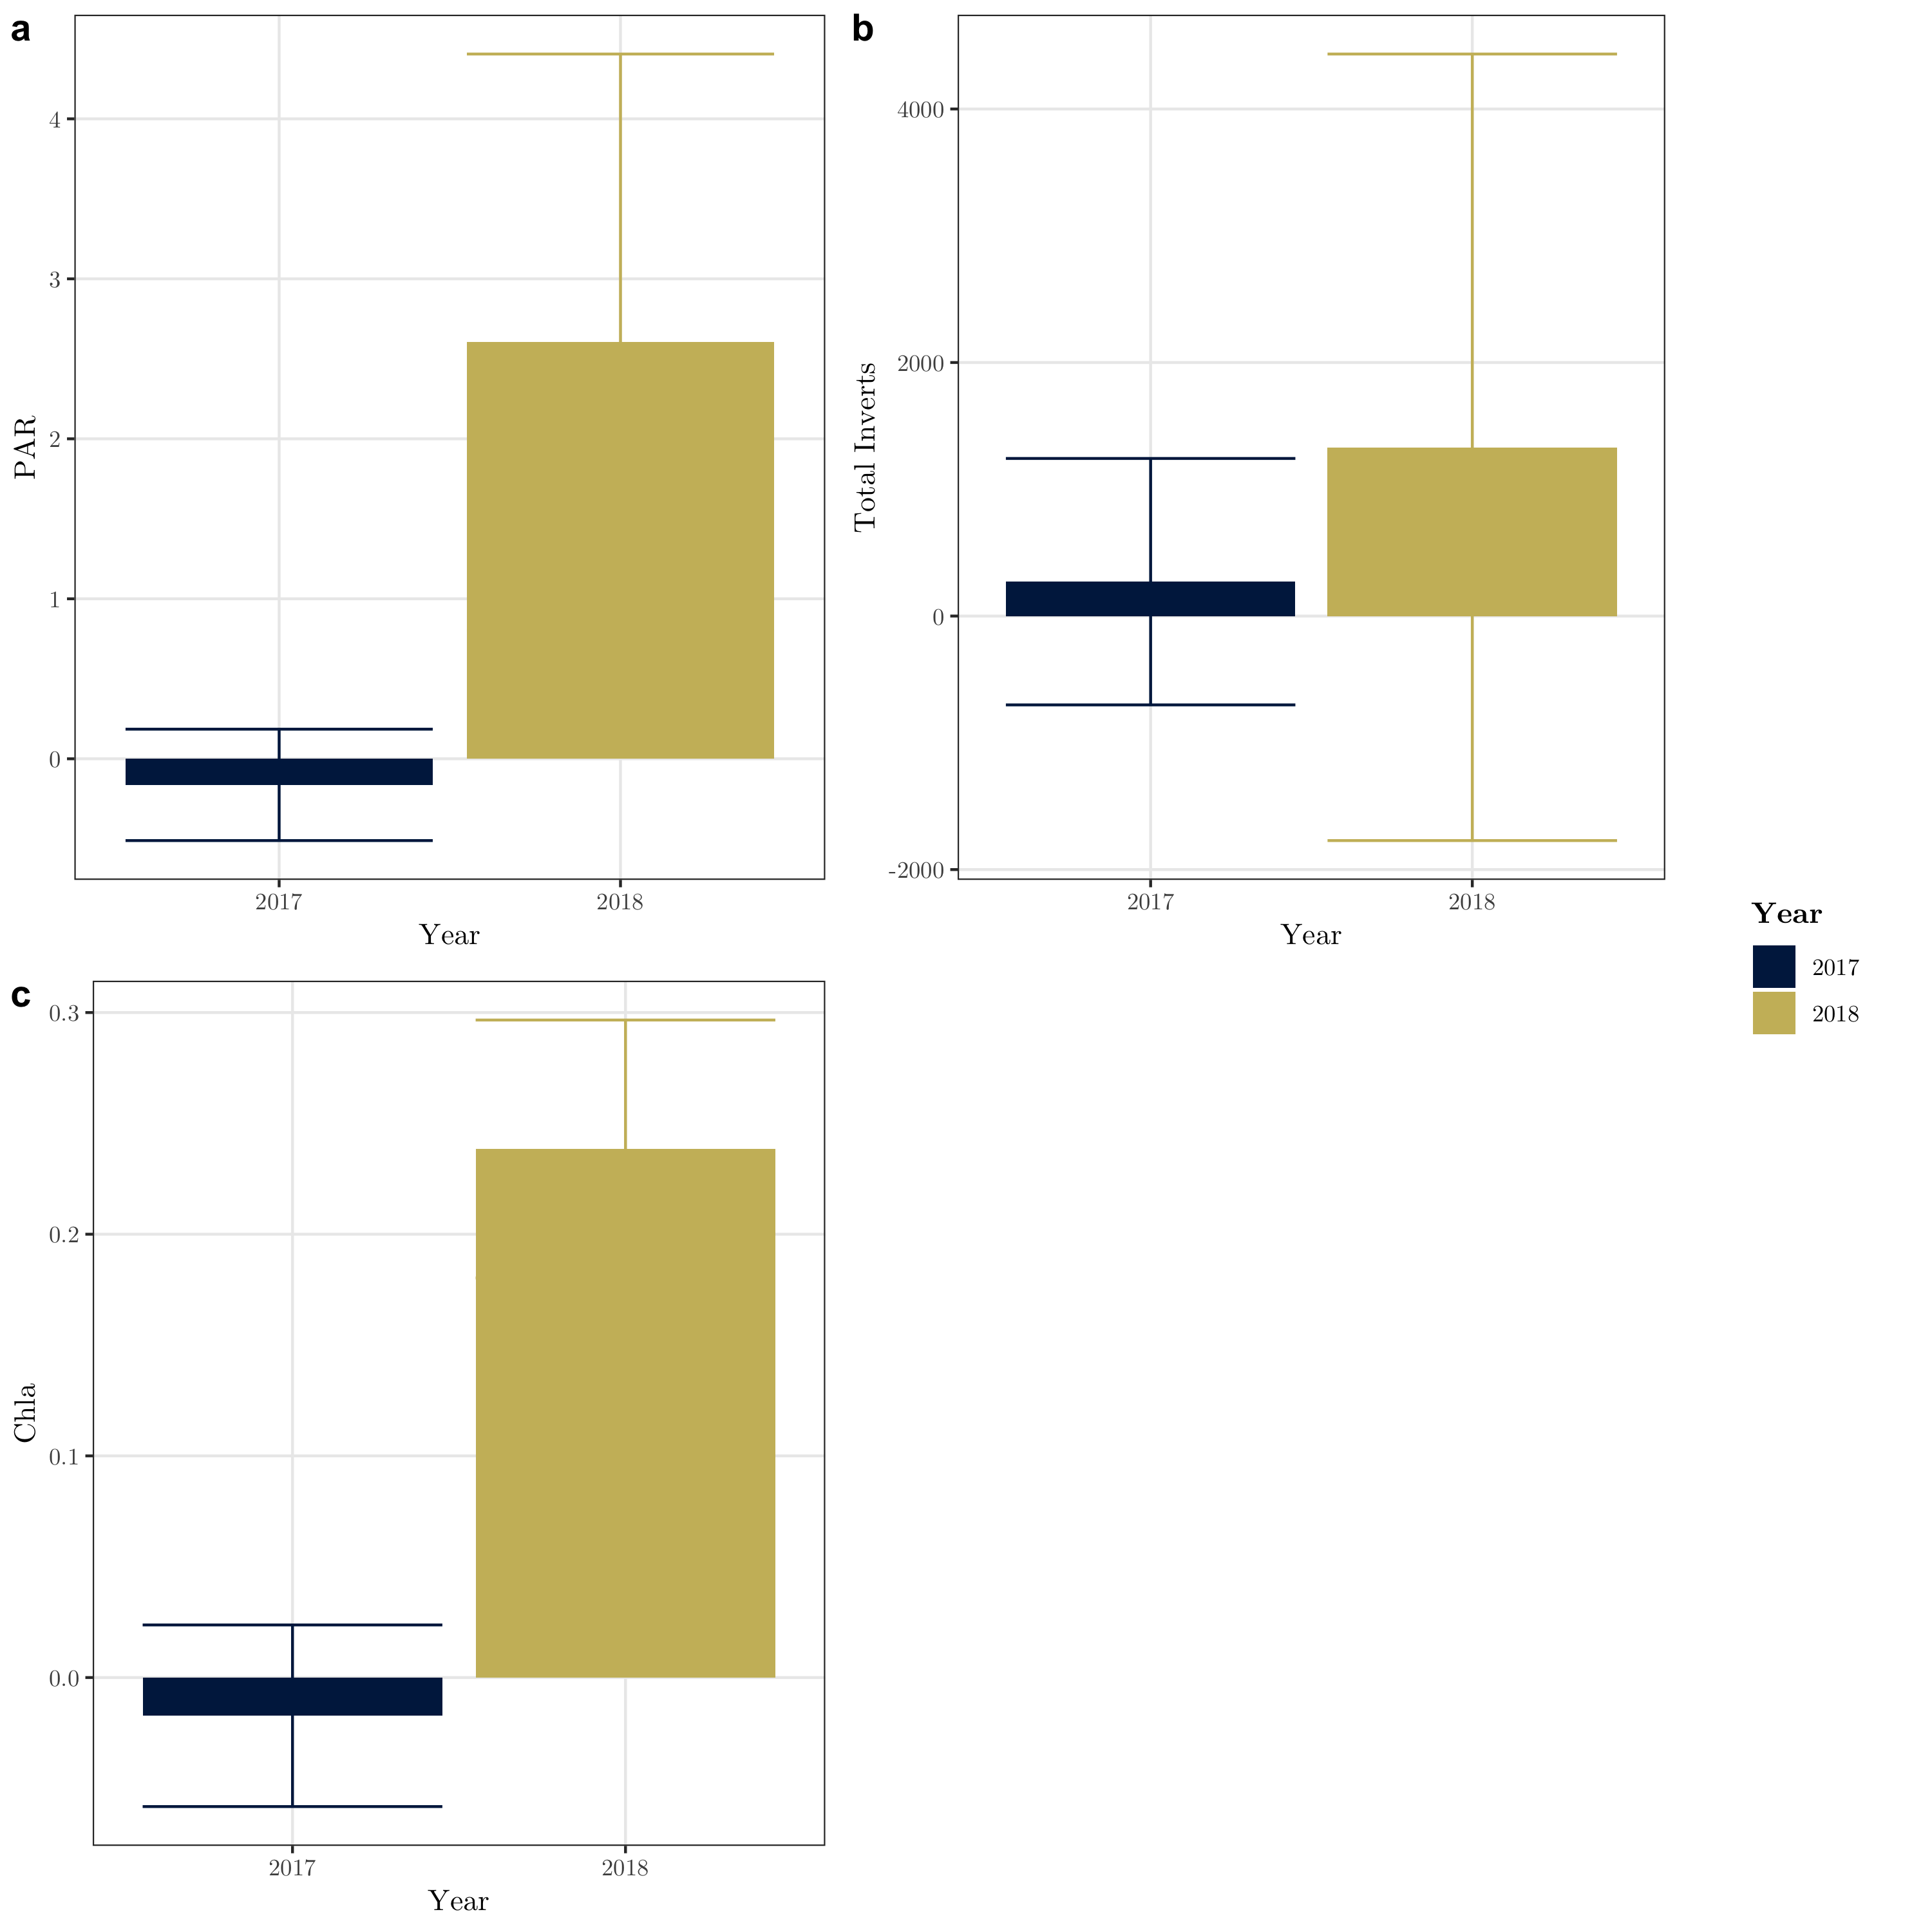
\includegraphics[width=1\linewidth]{Figures/Vars_Reach_Diffs} 
  
  }
  
  \caption[Light, Chla, total invertebrate abundance, and EPT index reach differences in the pre and post-treament years with error bars of one standard error]{Light, Chla, total invertebrate abundance, and EPT index reach differences in the pre and post-treament years with error bars of one standard error. \label{Exp-vars}}\label{fig:unnamed-chunk-1}
  \end{figure}
  
  As with light fluxes, prior to the experimental gap treatment, Chla,
  values across all sites in the pre-treatment year were low (mean = 0.095
  ug cm\textsuperscript{-2}), and there was little difference between
  reaches. After gaps were cut in the post-treatment year, Chla values
  went up by 0.44 ug cm\textsuperscript{-2} in the gap reach, and only
  0.175 ug cm\textsuperscript{-2} in the reference reach (final BACI
  difference = 0.265 ug cm\textsuperscript{-2}, p-value = 0.002).
  
  \begin{figure}
  
  {\centering 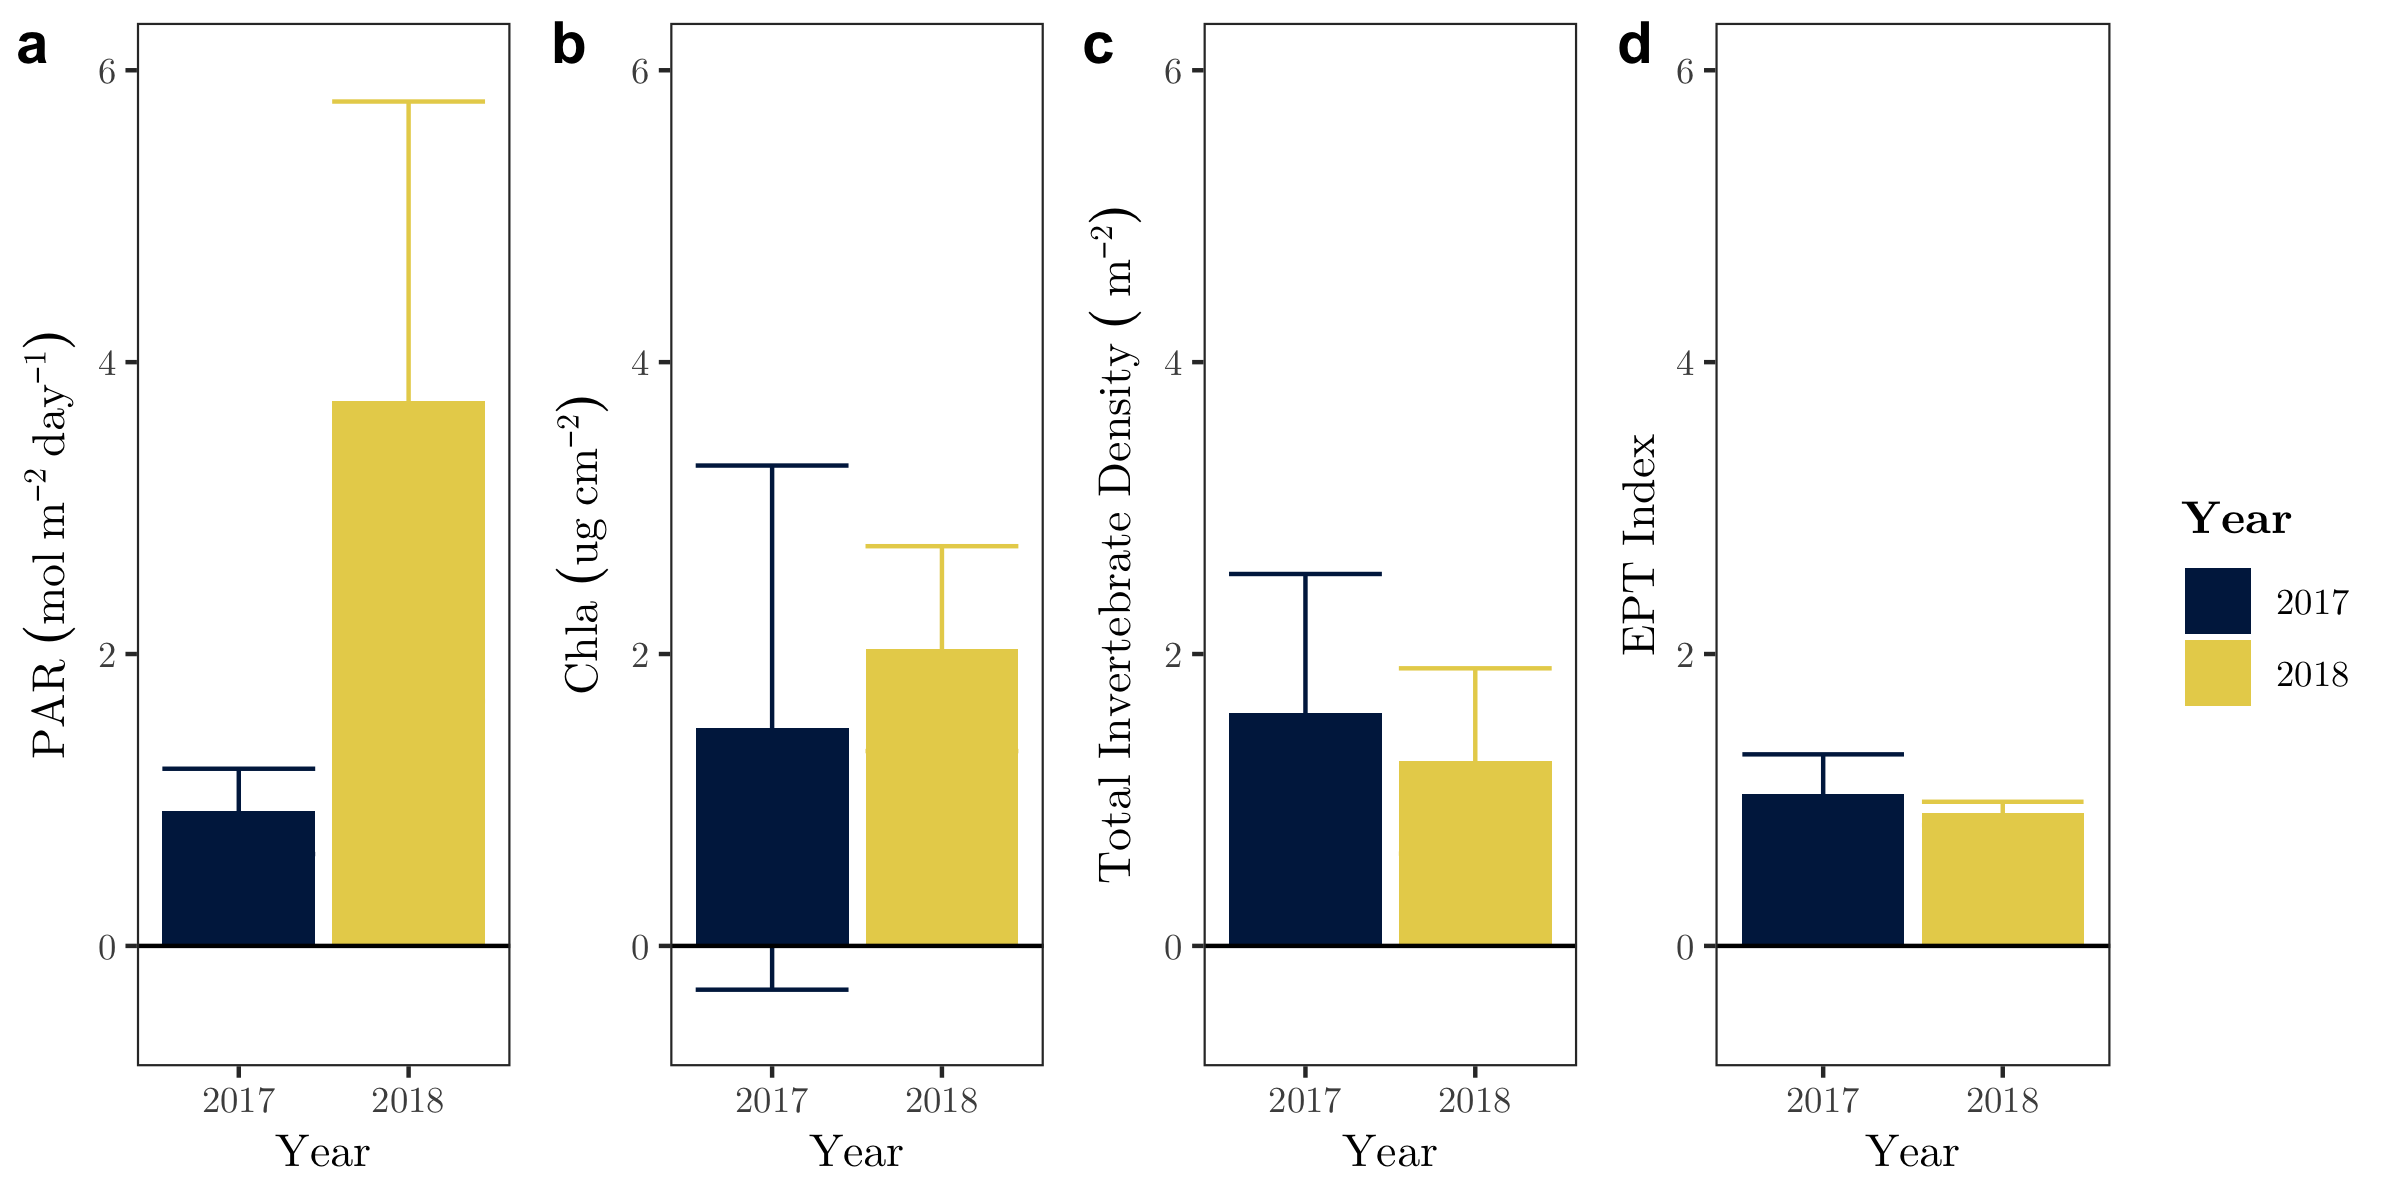
\includegraphics[width=1\linewidth]{Figures/Vars_Reach_rat} 
  
  }
  
  \caption[Light, Chla, total invertebrate abundance, and EPT index log ratio in the pre and post-treament years with error bars of one standard error]{Light, Chla, total invertebrate abundance, and EPT index log ratio in the pre and post-treament years with error bars of one standard error. \label{Exp-vars-rat}}\label{fig:unnamed-chunk-2}
  \end{figure}
  
  \section*{\texorpdfstring{\emph{Juga} on
  Tiles}{Juga on Tiles}}\label{juga-on-tiles}
  \addcontentsline{toc}{section}{\emph{Juga} on Tiles}
  
  In the pre-treatment year, the average density of \emph{Juga} on tiles
  among the two streams with \emph{Juga} present was 24.44 snails per
  m\textsuperscript{2} with little difference between the control and
  treatment reaches. In the post treatment year the average snail density
  in the treatment reach increased by 204.44 snails per
  m\textsuperscript{2}, whereas snail density in the control reach only
  increased by 88.89 snails per m\textsuperscript{2}. Snail abundance at
  these two streams was moderately associated with Chla
  (r\textsuperscript{2} = 0.32, p = 0.005), but saw the largest BACI
  response in meters ten and twenty, slightly upstream of the gap
  treatment.
  
  \section*{Benthic Invertebrate
  Community}\label{benthic-invertebrate-community}
  \addcontentsline{toc}{section}{Benthic Invertebrate Community}
  
  The density of Ephemeroptera, Plecoptera and Trichoptera relative to
  other taxa (the EPT index) did not change appreciably between years, and
  there was little difference between benthic invertebrate communities in
  the treatment and reference reaches in the pre-treatment year (MRBP: A =
  0.041, p = 0.071), or the post-treatment year (A = -0.022, p = 0.838).
  The indicator species analysis confirmed the lack of grouping from MRBP
  by not identifying any taxa with significant changes in fidelity or
  exclusivity in response to the treatment. The results from the NMS
  ordinations support the results of the MRBP and ISA (Figure 3) with
  community differences between years but not between reaches in either
  year.
  
  The NMS ordination of benthic invertebrates converged on a 2D solution
  with a final stress of 12.03. Chla (total chlorophyll values from the
  BenthoTorch) and PAR both had positive r\textsuperscript{2} values with
  axis 1 (PAR r\textsuperscript{2} = 0.45, Chla r\textsuperscript{2} =
  0.60). The main taxa driving the ordination are summarized in table 2.
  Chironomidae are a significant contributor to axis 1 (r = 0.83), while
  Heptageniidae have the strongest relationship with axis 2 (r = 0.73).
  
  \begin{figure}
  
  {\centering 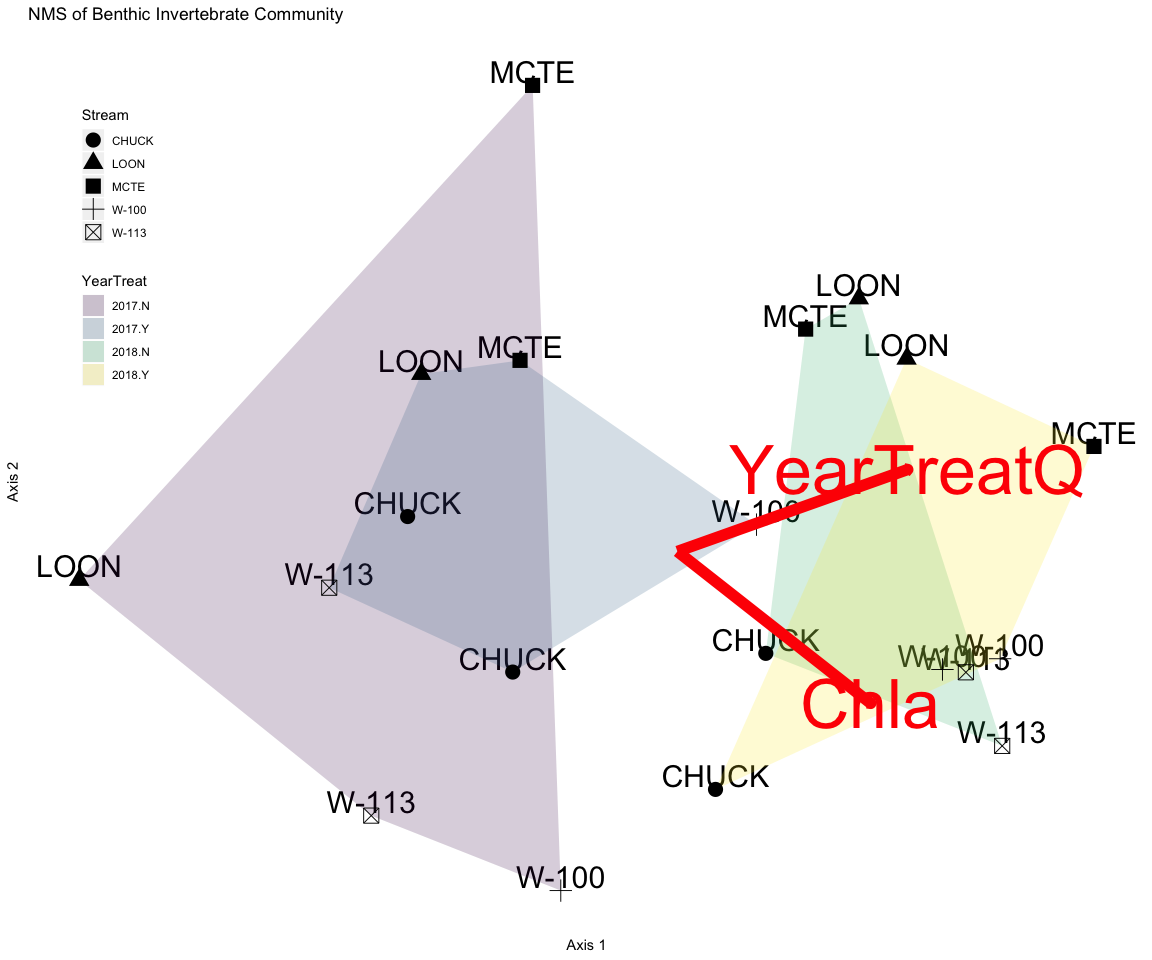
\includegraphics[width=1\linewidth]{Figures/NMS-Benthic-1} 
  
  }
  
  \caption[NMS of each reach in invertebrate community space]{NMS of each reach in invertebrate community space. Each point represents a single stream reach. Shapes identify stream and color identifies treament and year. The environmental vectors Chla and PAR were regressed against the synthetic community axis variables and overlaid on the plot. The length of the vectors indicate the strength of the relationship.}\label{fig:unnamed-chunk-3}
  \end{figure}
  
  \begin{table}[t]
  
  \caption{\label{tab:nmstable}Taxa with the greatest correlation with NMS ordination axis scores and p-value less than 0.05.}
  \centering
  \begin{tabular}{lrrr}
  \toprule
  Taxa & Axis 1 & Axis 2 & p-value\\
  \midrule
  Ampumixis & 0.24 & -0.58 & 0.02\\
  Baetis & 0.20 & -0.59 & 0.03\\
  Calineuria & 0.59 & -0.66 & 0.00\\
  Ceratapogonidae & 0.61 & 0.19 & 0.01\\
  Chironomidae & 0.83 & -0.26 & 0.00\\
  \addlinespace
  Elmidae & 0.21 & -0.57 & 0.03\\
  Glossosoma & 0.60 & -0.42 & 0.00\\
  Heptageniidae & 0.43 & -0.73 & 0.00\\
  Juga & 0.42 & -0.48 & 0.01\\
  Lara & 0.31 & -0.51 & 0.03\\
  \addlinespace
  Leuctridae & 0.58 & -0.33 & 0.01\\
  Mite & 0.52 & 0.67 & 0.00\\
  Paraleptophlebia & 0.19 & 0.63 & 0.01\\
  Rhyacophila & 0.41 & -0.55 & 0.01\\
  Tipulidae & 0.45 & 0.51 & 0.01\\
  \addlinespace
  Yoraperla & 0.02 & 0.60 & 0.02\\
  Zapada & 0.58 & 0.20 & 0.03\\
  \bottomrule
  \end{tabular}
  \end{table}
  
  \section*{Invertebrate Functional Feeding
  Groups}\label{invertebrate-functional-feeding-groups}
  \addcontentsline{toc}{section}{Invertebrate Functional Feeding Groups}
  
  Collector-gatherers were by far the most abundant functional feeding
  group in the post-treatment year for both reaches at all sites. This
  does not appear to be due to the treatment of the gaps since we see
  heightened collector-gatherer response in the reference reach as well.
  Collector-filterers were typically the least abundant FFG in any stream
  or year. No FFG had a significant response across all streams. Scraping
  invertebrates only showed a positive response to the gap in MCTE with
  all other streams having a moderately negative BACI response. When we
  treat streams as independent replicates and perform a t-test of total
  invertebrate density response and the density response of each FGG
  individually, we find that collector filterers did have a statistically
  significant response, but no other FFG had a consistent or significant
  response to the gap treatment (Table 3).
  
  \begin{figure}
  
  {\centering 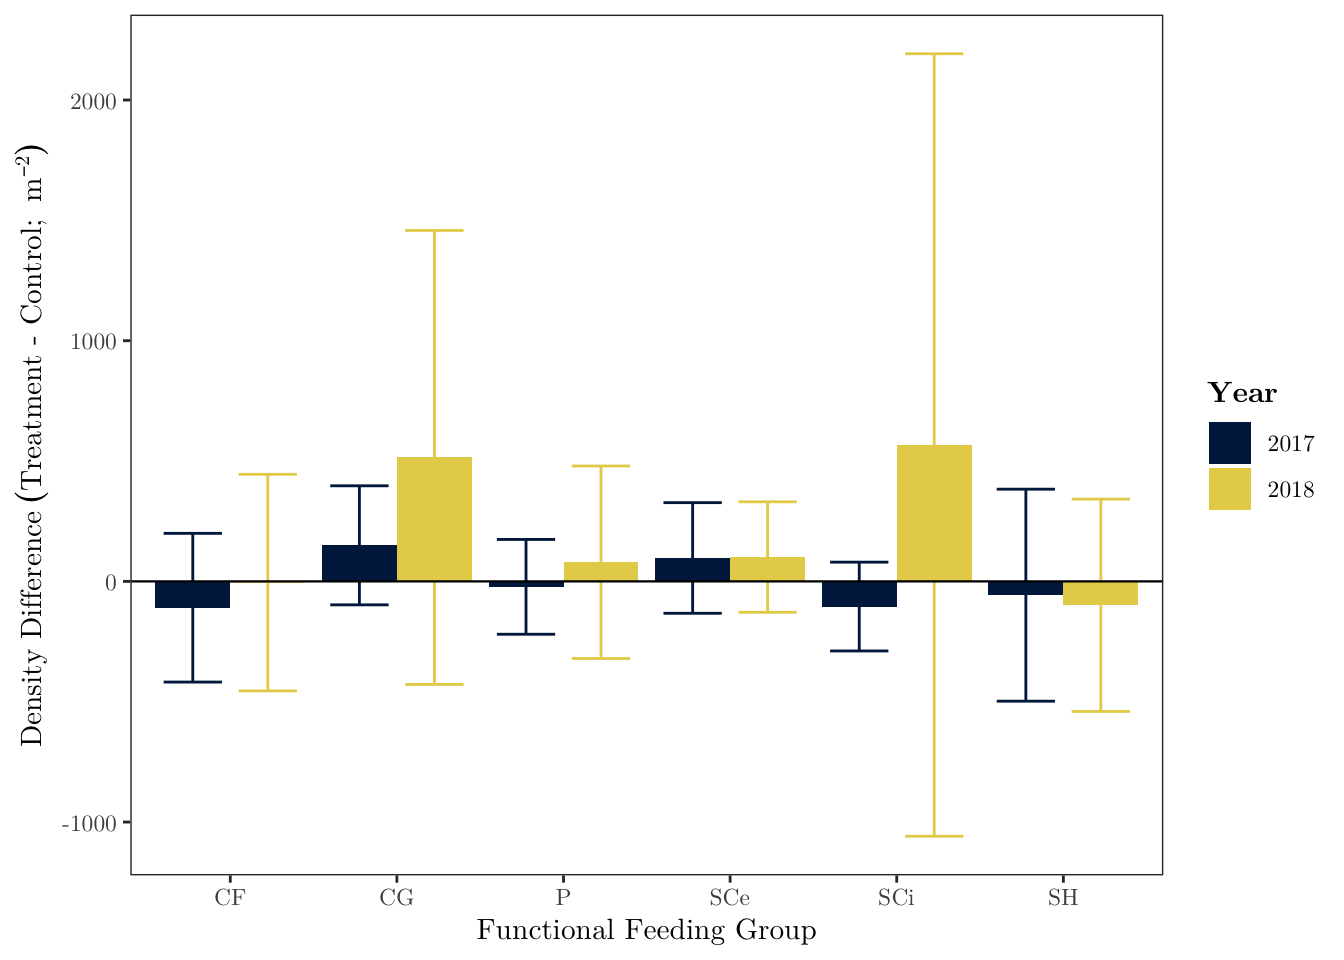
\includegraphics[width=1\linewidth]{Figures/AvgFFGdiff} 
  
  }
  
  \caption[Average reach difference of invertebrate density for each FFG with confidence intervals of one standard error]{Average reach difference of invertebrate density for each FFG with confidence intervals of one standard error. Negative values indicate higher abundance in the control reach on average, whereas positive values show higher abundance in the treatment reach. CF = Collector-filterer, CG = Collector-gatherer, P = Predators, SCe = Edible Scrapers, SCi = Inedible Scrapers, SH = Shredder.}\label{fig:unnamed-chunk-4}
  \end{figure}
  
  \begin{table}[t]
  
  \caption{\label{tab:ffgtable}Benthic invertebrate FFG responses t-test results. Collector gatherers are the only group with a statistically significant response.}
  \centering
  \begin{tabular}{lrr}
  \toprule
  FFG & t-value & p-value\\
  \midrule
  SH & 0.07 & 0.95\\
  P & 0.52 & 0.62\\
  SCe & -1.55 & 0.16\\
  CG & 0.60 & 0.57\\
  SCi & 0.86 & 0.42\\
  \addlinespace
  CF & 2.13 & 0.07\\
  All Bugs & 0.84 & 0.43\\
  \bottomrule
  \end{tabular}
  \end{table}
  
  \section*{Trout Diet}\label{trout-diet}
  \addcontentsline{toc}{section}{Trout Diet}
  
  The most common diet items were benthic invertebrates. Terrestrial
  invertebrates comprised between 25 and 86\% of fish diets across the
  five streams (Table 4). Overall, there was large stream-to-stream
  variations in trout diet selectivity (diet composition relative to
  benthic sample abundance), but in evaluating potential canopy gap
  effects, trout diet selectivity in the post treatment year did not vary
  significantly between reaches when assessing diets based on taxa
  (benthic invertebrates identified to family). When considering
  functional feeding groups in the diet, the largest difference between
  reaches in the difference selection index was predatory invertebrates
  (t-value = 1.043, p-value = 0.33) such as caddisfly of the family
  Rhyacophilidae.
  
  \begin{figure}
  
  {\centering 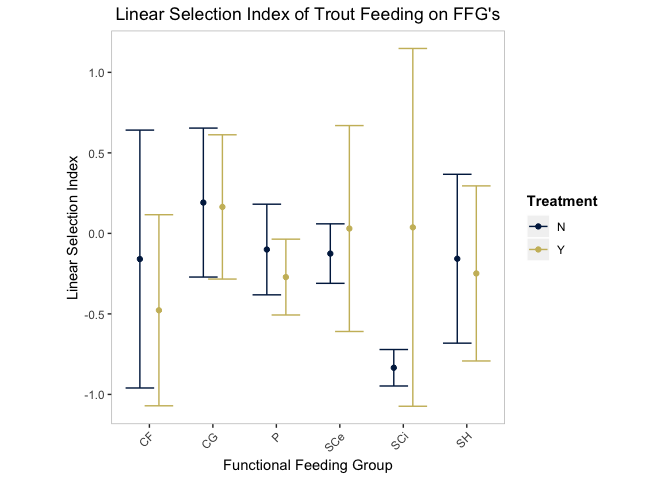
\includegraphics[width=1\linewidth]{Figures/Diet-FFG-D-1} 
  
  }
  
  \caption[Linear selection index of trout diet samples]{Linear selection index of trout diet samples. Values close to zero indicate opportunistic foraging strategies where trout consume prey directly proportional to their abundance in the environment. Positive values show preferential consumption and negative values are prey items consumed less than expected based on their abundance in the environment.}\label{fig:unnamed-chunk-5}
  \end{figure}
  
  \begin{table}[t]
  
  \caption{\label{tab:dietffg}Proportional abundances of each FFG and terrestrial invertebrates for each site.}
  \centering
  \begin{tabular}{lrrrrr}
  \toprule
  FFG & LOON & CHUCK & MCTE & W-100 & W-113\\
  \midrule
  CF & 0.07 & 0.03 & 0.06 & 0.06 & 0.03\\
  CG & 0.32 & 0.28 & 0.33 & 0.32 & 0.04\\
  P & 0.18 & 0.08 & 0.06 & 0.08 & 0.04\\
  SCe & 0.05 & 0.03 & 0.04 & 0.05 & 0.02\\
  Sci & 0.00 & 0.02 & 0.04 & 0.01 & 0.00\\
  \addlinespace
  SH & 0.13 & 0.20 & 0.14 & 0.04 & 0.03\\
  Terr. & 0.25 & 0.36 & 0.33 & 0.44 & 0.86\\
  \bottomrule
  \end{tabular}
  \end{table}
  
  At the family level, trout diets remained variable in composition. The
  family with the greatest variability in trout diets was \emph{Juga}
  snails with two trout in MCTE showing strong selection (Table 5) and all
  other trout consistently avoiding snails.
  
  \begin{table}[t]
  
  \caption{\label{tab:TopDiet}Most abundant taxa in trout diets across streams. Note the high representation of Juga snails in the diets of trout at MCTE.}
  \centering
  \begin{tabular}{lrrrrr}
  \toprule
  Family & CHUCK & LOON & MCTE & W-100 & W-113\\
  \midrule
  Baetidae & 0.355 & 0.295 & 0.205 & 0.172 & 0.542\\
  Brachycentridae & 0.137 & 0.693 & 0.193 & 0.049 & 0.000\\
  Chironomidae & 0.670 & 0.381 & 0.337 & 0.421 & 0.167\\
  Dixidae & 0.061 & 0.000 & 0.048 & 0.122 & 0.111\\
  Elmidae & 0.054 & 0.000 & 0.072 & 0.249 & 0.000\\
  \addlinespace
  Ephemerellidae & 0.048 & 0.125 & 0.036 & 0.049 & 0.000\\
  Heptageniidae & 0.038 & 0.000 & 0.036 & 0.174 & 0.236\\
  Hydropsychidae & 0.032 & 0.000 & 0.000 & 0.049 & 0.181\\
  Juga & 0.000 & 0.045 & 0.482 & 0.024 & 0.000\\
  Leptophlebiidae & 0.000 & 0.000 & 0.084 & 0.049 & 0.000\\
  \addlinespace
  Ostrocod & 0.077 & 0.091 & 0.145 & 0.050 & 0.000\\
  Perlidae & 0.198 & 0.045 & 0.036 & 0.024 & 0.111\\
  Rhyacophilidae & 0.176 & 0.153 & 0.012 & 0.123 & 0.236\\
  Simuliidae & 0.022 & 0.012 & 0.036 & 0.073 & 0.125\\
  Tipulidae & 0.022 & 0.000 & 0.036 & 0.150 & 0.181\\
  \bottomrule
  \end{tabular}
  \end{table}
  
  \chapter*{Discussion}\label{discussion}
  \addcontentsline{toc}{chapter}{Discussion}
  
  Gaps are, by definition, open canopy patches in a larger forested
  system. While localized responses beneath a gap may occur, we were
  particularly interested in whether the effect of an individual canopy
  gap could be detected at the stream reach scale. Studies have found that
  large-scale removal of forest canopies along an entire stream reach
  (Wootton, \protect\hyperlink{ref-Wootton2012}{2012}), or patches of high
  shade (Heaston, Kaylor, \& Warren,
  \protect\hyperlink{ref-Heaston2018}{2018}), had an effect on the overall
  invertebrate community. Yet, significant localized responses within a
  single gap may not translate to significant system-wide responses at the
  stream or even the reach level. Our study design emphasizes the effects
  of gaps that only comprise a fraction of a stream reach, so the focus is
  placed on the integrated effect of small gaps embedded in a larger
  forested environment. Benthic algae increased as expected in the
  localized areas under a gap, but we were particularly interested in
  understanding whether anticipated local increases in benthic algae
  extended to reach-scale increases in benthic macroinvertebrates. Across
  five replicate streams on which we cut experimental canopy gaps, benthic
  algae increased as expected, but overall there were few clear responses
  in the macroinvertebrate community. Further, through an assessment of
  fish diet, we ruled out the possibility that fish were selectively
  feeding on a given taxa group or functional feeding group in response to
  the gaps and thereby masking a potential response in a subset of the
  benthic invertebrate community.
  
  While the canopy-opening treatments increased PAR by as much as
  \(400\%\), they were not outside the realm of what could occur naturally
  in these heavily shaded systems. Though these small-scale distrubances
  significantly increase abiotic factors such as light, the localized
  impact of light increases on stream biota did not manifest at the reach
  level. Trophic inefficiency or changes in the algal community in
  response to more saturated light conditions (Lesutienė, Gorokhova,
  Stankevičienė, Bergman, \& Greenberg,
  \protect\hyperlink{ref-Lesutiene2014}{2014}) may explain the dwindling
  returns in production from primary producers to consumers as seen in
  figure 2. But, we also saw muted responses in primary production
  compared to previous studies on photosynthesis and light conditions that
  indicate a strong linear relationship between light and GPP at light
  levels lower than two hundred \(\mu\)mol m\textsuperscript{-2s}-1
  (Boston \& Hill, \protect\hyperlink{ref-Boston1991}{1991}). Our
  increases in PAR were concentrated to a relatively small area, and it is
  possible that algae within the gaps were experiencing photosaturation
  limitations, or faced nutrient co-limitations.
  
  Overall, our invertebrate communities had greater variability between
  streams than between treatment reaches, and no taxa have a consistent
  response across sites. Because the macroinvertebrate community varied
  substantially across streams, we felt that it was also important to
  explore functional feeding group responses. For example, we expected to
  see a response of scraping invertebrates in response to greater benthic
  algal abundances, even if those were manifesting across different taxa
  that feed on a similar food source. While there has been some
  controversy surounding the use of functional feeding groups to directly
  infer food being consumed (Rosi-Marshall, Vallis, Baxter, \& Davis,
  \protect\hyperlink{ref-Rosi2016}{2016}), within the scope of our
  hypothesis, and given the varied community response across sites, we
  felt justified in using functional feeding groups as an additional tool
  to explore responses in the invertebrate community to increased
  light--and associated increases in benthic algae.
  
  Our functional feeding group results at the reach-level seem to be in
  contradiction with previous studies on stream light (Heaston et al.,
  \protect\hyperlink{ref-Heaston2018}{2018}; Kaylor \& Warren,
  \protect\hyperlink{ref-Kaylor2017Eco}{2017}; Wootton,
  \protect\hyperlink{ref-Wootton2012}{2012}), but these studies focused on
  the immediate, within-treatment response of invertebrates and fish to
  various alterations to light availability. While we did not see
  significant reach-scale differences in secondary macroinvertebrate
  production, there was a localized \emph{Juga} snail response in meters
  adjacent to the gap. It may be that the sessile life history strategy of
  \emph{Juga} allows them to take advantage of localized increases in
  productivity without being washed downstream like other more motile
  taxa. In that regard, our snails responded locally as expected, but the
  relative size of our canopy manipulations, one similar to small-scale
  natural disturbances and individual tree mortality, limited reach-level
  trophic responses.
  
  When tracing energy flows through an aquatic food chain, stable isotope
  analysis can reveal the source carbon in higher trophic levels and lend
  insight into the net autotrophy of the system. However, community
  studies have the potential to reveal more subtle patterns in energy
  transfer. For example, snails and other heavily armored scrapers may
  effectively sequester autocthonous carbon from higher trophic levels
  (Power \& Dietrich, \protect\hyperlink{ref-Power2002}{2002}). In our
  trout diets, we found strong support for the inedibility of snails and
  cased caddisfly larvae with the exception of Brachycentrid caddisflies.
  Yet, there was no significant difference in selection pressure between
  reaches to explain the general lack of a scraper response to increased
  algal productivity in the treatment reach, even among these taxa that
  experience less top-down pressure.
  
  In general, fish diets were variable with no clear preference or
  avoidance of any one FFG or taxa group found consistently across
  streams. A scraper response is most likely not being masked by selective
  trout foraging because we did not find a significant top-down pressure
  on scraping invertebrates. However, our trout diets only provide a
  snapshot of trout foraging from a single day in mid-summer. The
  differing life histories of benthic invertebrates may expose them to
  varying top-down pressure throughout the year that are not accurately
  captured in this study. Compared to other studies in the region (Romero,
  Gresswell, \& Li, \protect\hyperlink{ref-Romero2005}{2005}), our trout
  diets were relatively sparse with half the diet items on average for
  summer trout diets.
  
  Determining a per-unit-light biotic response is complicated by complex
  trophic dynamics and limits on primary productivity such as
  photosaturation and nutrient limitation. Canopy-opening manipulations
  designed to mimic the patchy light environment of old-growth systems and
  stimulate productivity in heavily shaded systems must account for these
  inherent, dampening, system complexities. Past studies demonstrate clear
  differences between old-growth and regenerating forest light dynamics
  and system productivity, but our single-gap study produced little biotic
  response. More or larger gaps may be necessary to create system-wide
  change.
  
  Studies on clearing hundreds of meters of riparian vegetation {[}Wootton
  (\protect\hyperlink{ref-Wootton2012}{2012}); Roon, unpublished data{]}
  demonstrated several-fold increases in primary production along with
  increases in primary consumers such as invertebrates. However, increases
  in temperature above the threshhold for many salmonids is not uncommon.
  Whether future management is intent on accelerating the progression
  toward old-growth forest structure and function or on increasing overall
  productivity of forest and stream systems, creating a dynamic light
  environment that strikes a balance between deleterious temperature
  increases and optimum system functioning may hinge on the patchy light
  pattern of canopy gaps.
  
  \pagebreak
  
  \chapter*{References}\label{references}
  \addcontentsline{toc}{chapter}{References}
  
  \setlength{\parindent}{-0.2in} \setlength{\leftskip}{0.2in}
  \setlength{\parskip}{8pt} \noindent
  
  \hypertarget{refs}{}
  \hypertarget{ref-Bechtold2012}{}
  Bechtold, H. A., Rosi-Marshall, E. J., Warren, D. R., \& Cole, J. J.
  (2012). A practical method for measuring integrated solar radiation
  reaching streambeds using photodegrading dyes. \emph{Freshwater
  Science}, \emph{31}(4), 1070--1077.
  
  \hypertarget{ref-Boston1991}{}
  Boston, H., \& Hill, W. (1991). Photosynthesis--light relations of
  stream periphyton communities. \emph{Limnology and Oceanography},
  \emph{36}(4), 644--656.
  
  \hypertarget{ref-Cole2003}{}
  Cole, M. B., Russell, K. R., \& Mabee, T. J. (2003). Relation of
  headwater macroinvertebrate communities to in-stream and adjacent stand
  characteristics in managed second-growth forests of the oregon coast
  range mountains. \emph{Canadian Journal of Forest Research},
  \emph{33}(8), 1433--1443.
  
  \hypertarget{ref-Dahl1998}{}
  Dahl, J. (1998). The impact of vertebrate and invertebrate predators on
  a stream benthic community. \emph{Oecologia}, \emph{117}(1-2), 217--226.
  
  \hypertarget{ref-Heaston2018}{}
  Heaston, E. D., Kaylor, M. J., \& Warren, D. R. (2018). Aquatic food web
  response to patchy shading along forested headwater streams.
  \emph{Canadian Journal of Fisheries and Aquatic Sciences},
  \emph{75}(12), 2211--2220.
  
  \hypertarget{ref-Jacobs1974}{}
  Jacobs, J. (1974). Quantitative measurement of food selection.
  \emph{Oecologia}, \emph{14}(4), 413--417.
  
  \hypertarget{ref-Kaylor2017Eco}{}
  Kaylor, M. J., \& Warren, D. R. (2017). Linking riparian shade and the
  legacies of forest management to fish and vertebrate biomass in forested
  streams. \emph{Ecosphere}, \emph{8}(6), e01845.
  
  \hypertarget{ref-Kaylor2018}{}
  Kaylor, M. J., Argerich, A., White, S. M., VerWey, B. J., \& Arismendi,
  I. (2018). A cautionary tale for in situ fluorometric measurement of
  stream chlorophyll a: Influences of light and periphyton biomass.
  \emph{Freshwater Science}, \emph{37}(2), 287--295.
  
  \hypertarget{ref-Kaylor2017FS}{}
  Kaylor, M. J., Warren, D. R., \& Kiffney, P. M. (2017). Long-term
  effects of riparian forest harvest on light in pacific northwest (USA)
  streams. \emph{Freshwater Science}, \emph{36}(1), 1--13.
  
  \hypertarget{ref-Kreutzweiser2012}{}
  Kreutzweiser, D. P., Sibley, P. K., Richardson, J. S., \& Gordon, A. M.
  (2012). Introduction and a theoretical basis for using disturbance by
  forest management activities to sustain aquatic ecosystems.
  \emph{Freshwater Science}, \emph{31}(1), 224--231.
  
  \hypertarget{ref-Kruskal1964}{}
  Kruskal, J. B. (1964). Multidimensional scaling by optimizing goodness
  of fit to a nonmetric hypothesis. \emph{Psychometrika}, \emph{29}(1),
  1--27.
  
  \hypertarget{ref-Lau2009}{}
  Lau, D. C. P., Leung, K. M. Y., \& Dudgeon, D. (2009). What does stable
  isotope analysis reveal about trophic relationships and the relative
  importance of allochthonous and autochthonous resources in tropical
  streams? A synthetic study from hong kong. \emph{Freshwater Biology},
  \emph{54}(1), 127--141.
  
  \hypertarget{ref-Lesutiene2014}{}
  Lesutienė, J., Gorokhova, E., Stankevičienė, D., Bergman, E., \&
  Greenberg, L. (2014). Light increases energy transfer efficiency in a
  boreal stream. \emph{PloS One}, \emph{9}(11), e113675.
  
  \hypertarget{ref-liess2012}{}
  Liess, A., Le Gros, A., Wagenhoff, A., Townsend, C. R., \& Matthaei, C.
  D. (2012). Landuse intensity in stream catchments affects the benthic
  food web: Consequences for nutrient supply, periphyton c: Nutrient
  ratios, and invertebrate richness and abundance. \emph{Freshwater
  Science}, \emph{31}(3), 813--824.
  
  \hypertarget{ref-Macarelli2011}{}
  Macarelli, A. M., Baxter, C. V., Mineau, M. M., \& Hall Jr, R. O.
  (2011). Quantity and quality: Unifying food web and ecosystem
  perspectives on the role of resource subsidies in freshwater.
  \emph{Ecology}, \emph{92}, 1215--1225.
  
  \hypertarget{ref-PC-ORD}{}
  McCune, B., \& Mefford, M. J. (2016). \emph{PC-ord. multivariate
  analysis of ecological data. version 7.} Gleneden Beach, Oregon, U.S.A.:
  MjM Software Design.
  
  \hypertarget{ref-McCune2002}{}
  McCune, B., Grace, J. B., \& Urban, D. L. (2002). \emph{Analysis of
  ecological communities} (Vol. 28). MjM software design Gleneden Beach,
  OR.
  
  \hypertarget{ref-McCutchan2002}{}
  McCutchan, J. H. J., \& Lewis, W. M. J. (2002). Relative importance of
  carbon sources for macroinvertebrates in a rocky mountain stream.
  \emph{Limnology and Oceanography}, \emph{47}(3), 742--752.
  
  \hypertarget{ref-Merritt2008}{}
  Merritt, R. W., Cummins, K. W., \& Berg, M. B. (2008). \emph{An
  introduction to the aquatic insects of north america}. Kendall Hunt.
  
  \hypertarget{ref-Murphy1981}{}
  Murphy, M. L., \& Hall, J. D. (1981). Vaired effects of clear-cut
  logging on predators and their habitat in small streams of the cascade
  mountains, oregon. \emph{Canadian Journal of Fisheries and Aquatic
  Sciences}, \emph{38}(2), 137--145.
  
  \hypertarget{ref-vegan}{}
  Oksanen, J., Blanchet, F. G., Friendly, M., Kindt, R., Legendre, P.,
  McGlinn, D., \ldots{} Wagner, H. (2018). \emph{Vegan: Community ecology
  package}. Retrieved from \url{https://CRAN.R-project.org/package=vegan}
  
  \hypertarget{ref-Pan2011}{}
  Pan, Y., Chen, J. M., Birdsey, R., McCullough, K., He, L., \& Deng, F.
  (2011). Age structure and disturbance legacy of north american forests.
  \emph{Biogeosciences. 8: 715-732.}, \emph{8}, 715--732.
  
  \hypertarget{ref-Peckarsky1998}{}
  Peckarsky, B. L., \& McIntosh, A. R. (1998). Fitness and community
  consequences of avoiding multiple predators. \emph{Oecologia},
  \emph{113}(4), 565--576.
  
  \hypertarget{ref-Power2002}{}
  Power, M. E., \& Dietrich, W. E. (2002). Food webs in river networks.
  \emph{Ecological Research}, \emph{17}(4), 451--471.
  
  \hypertarget{ref-Purcell2009}{}
  Purcell, A. H., Bressler, D. W., Paul, M. J., Barbour, M. T., Rankin, E.
  T., Carter, J. L., \& Resh, V. H. (2009). Assessment tools for urban
  catchments: Developing biological indicators based on benthic
  macroinvertebrates 1. \emph{JAWRA Journal of the American Water
  Resources Association}, \emph{45}(2), 306--319.
  
  \hypertarget{ref-R-base}{}
  R Core Team. (2018). \emph{R: A language and environment for statistical
  computing}. Retrieved from \url{https://www.R-project.org/}
  
  \hypertarget{ref-Romero2005}{}
  Romero, N., Gresswell, R. E., \& Li, J. L. (2005). Changing patterns in
  coastal cutthroat trout (oncorhynchus clarki clarki) diet and prey in a
  gradient of deciduous canopies. \emph{Canadian Journal of Fisheries and
  Aquatic Sciences}, \emph{62}(8), 1797--1807.
  
  \hypertarget{ref-Rosi2016}{}
  Rosi-Marshall, E. J., Vallis, K. L., Baxter, C. V., \& Davis, J. M.
  (2016). Retesting a prediction of the river continuum concept:
  Autochthonous versus allochthonous resources in the diets of
  invertebrates. \emph{Freshwater Science}, \emph{35}(2), 534--543.
  
  \hypertarget{ref-Vannote1980}{}
  Vannote, R. L., Minshall, G. W., Cummins, K. W., Sedell, J. R., \&
  Cushing, C. E. (1980). The river continuum concept. \emph{Canadian
  Journal of Fisheries and Aquatic Sciences}, \emph{37}(1), 130--137.
  
  \hypertarget{ref-Wallace1996}{}
  Wallace, J. B., Grubaugh, J. W., \& Whiles, M. R. (1996). Biotic indices
  and stream ecosystem processes: Results from an experimental study.
  \emph{Ecological Applications}, \emph{6}(1), 140--151.
  
  \hypertarget{ref-Warren2017}{}
  Warren, D. R., Collins, S. M., Purvis, E. M., Kaylor, M. J., \&
  Bechtold, H. A. (2017). Spatial variability in light yields colimitation
  of primary production by both light and nutrients in a forested stream
  ecosystem. \emph{Ecosystems}, \emph{20}(1), 198--210.
  
  \hypertarget{ref-Warren2013}{}
  Warren, D. R., Keeton, W. S., Bechtold, H. A., \& Rosi-Marshall, E. J.
  (2013). Comparing streambed light availability and canopy cover in
  streams with old-growth versus early-mature riparian forests in western
  oregon. \emph{Aquatic Sciences}, \emph{75}(4), 547--558.
  
  \hypertarget{ref-Warren2016Eco}{}
  Warren, D. R., Keeton, W. S., Kiffney, P. M., Kaylor, M. J., Bechtold,
  H. A., \& Magee, J. (2016). Changing forests---changing streams:
  Riparian forest stand development and ecosystem function in temperate
  headwaters. \emph{Ecosphere}, \emph{7}(8).
  
  \hypertarget{ref-Wilzbach1986}{}
  Wilzbach, M. A., Cummins, K. W., \& Hall, J. D. (1986). Influence of
  habitat manipulations on interactions between cutthroat trout and
  invertebrate drift. \emph{Ecology}, \emph{67}(4), 898--911.
  
  \hypertarget{ref-Wipfli1997}{}
  Wipfli, M. S. (1997). Terrestrial invertebrates as salmonid prey and
  nitrogen sources in streams: Contrasting old-growth and young-growth
  riparian forests in southeastern alaska, usa. \emph{Canadian Journal of
  Fisheries and Aquatic Sciences}, \emph{54}(6), 1259--1269.
  
  \hypertarget{ref-Wootton2012}{}
  Wootton, J. T. (2012). River food web response to large-scale riparian
  zone manipulations. \emph{PLoS One}, \emph{7}(12), e51839.


\end{document}

